
% additional usepackage{beamerthemeshadow} is used
\documentclass{beamer}
%\usepackage{beamerthemeshadow}

\usepackage{lmodern} % Font
\usepackage[T1]{fontenc} % Can use danish characters
\usepackage[utf8]{inputenc} %input encoding. Can be used on Linux, Mac and Windows         
\usepackage[english]{babel} %Split words accoding to English

\input{../Modules/Modules/FigureSetup}
\input{../Modules/Modules/URLSetup}

\begin{document}

\title{Version control and GitHub}  
\author{Rasmus Bækgaard}
\date{\today} 

\frame{
	\titlepage
	
	\begin{figure}[hbtp]
	\centering
	
\includegraphics[width=0.48\textwidth]{Octocat.png}
	\end{figure}
} 

\frame{\frametitle{Table of contents}\tableofcontents} 



\section{What is GitHub and what can it do?}
\frame
{
	\frametitle{What is GitHub and what can it do?}
	
\begin{itemize}
\item GitHub is a service which stores your files, makes them safe and 
accessible from you and your collaborator(s) computer(s).

\item This service can be used for the semester projects, bachelor project, 
course projects and projects you do in your free time.

\item GitHub uses Linus Torvals's program, Git, which Linus uses for the Linux 
kernel and Google uses for Android.

\item GitHub had in April 2014 +3.4 million users -- the biggest code host in 
the world.
\end{itemize}

}

\subsection{Example}
\frame{ 
	\frametitle{Why do you want to use it?}

	\begin{figure}[hbtp]
		\centering
		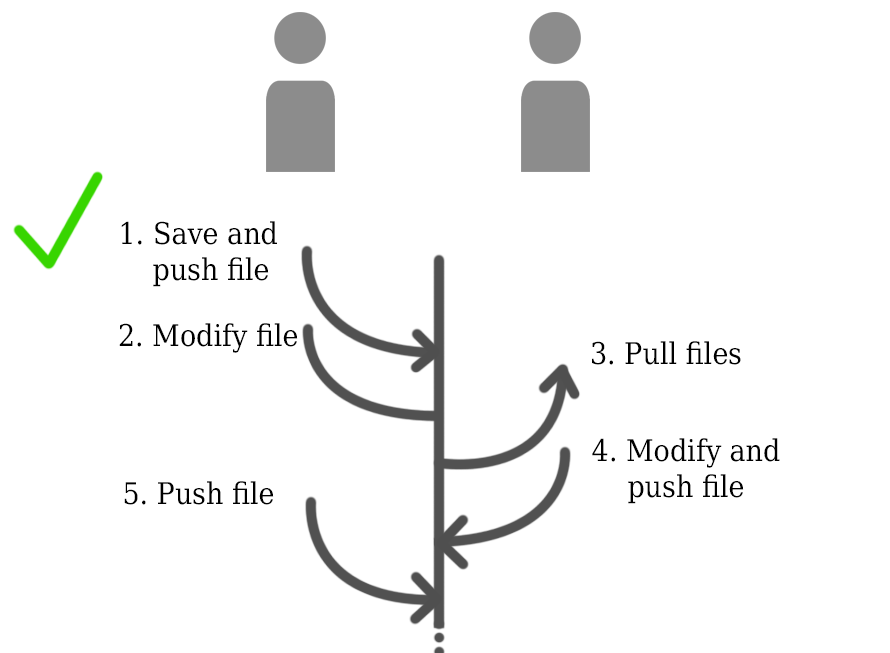
\includegraphics[width=0.9\textwidth]{VCS1}
	\end{figure}

}

\frame{ 
	\frametitle{Why do you want to use it?}
	
	\begin{figure}[hbtp]
		\centering
		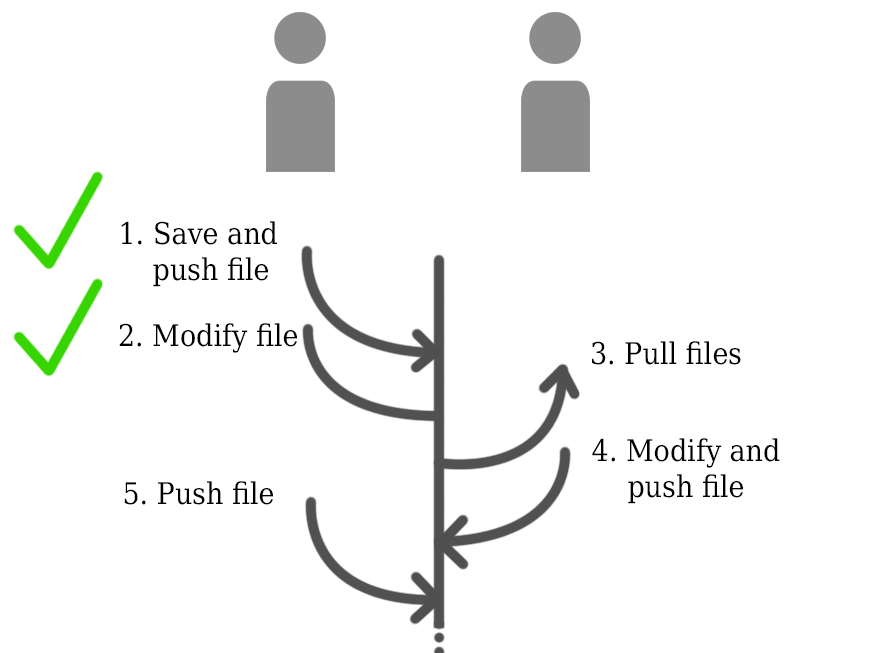
\includegraphics[width=0.9\textwidth]{VCS2}
	\end{figure}
	
}

\frame{ 
	\frametitle{Why do you want to use it?}
	
	\begin{figure}[hbtp]
		\centering
		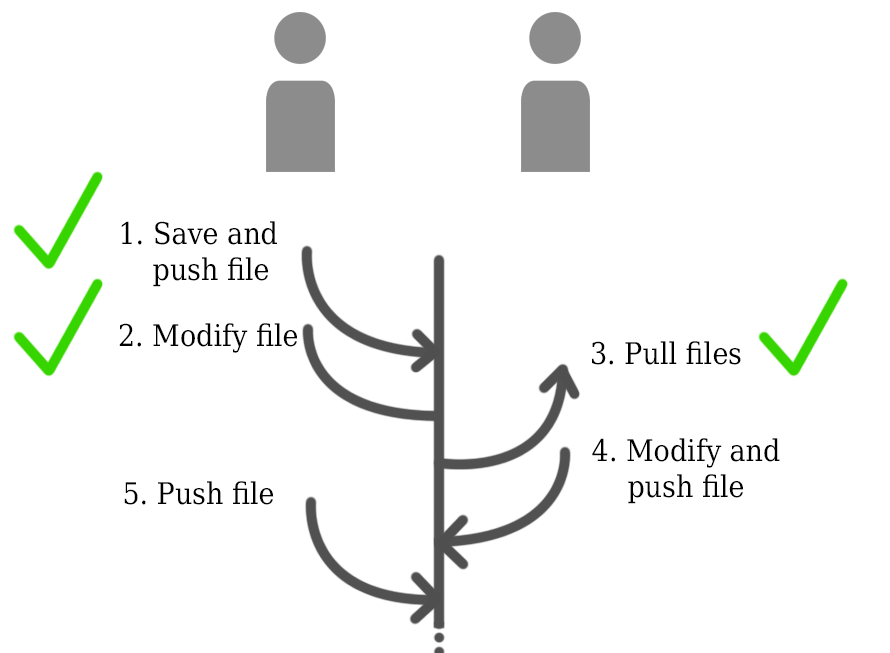
\includegraphics[width=0.9\textwidth]{VCS3}
	\end{figure}
	
}

\frame{ 
	\frametitle{Why do you want to use it?}
	
	\begin{figure}[hbtp]
		\centering
		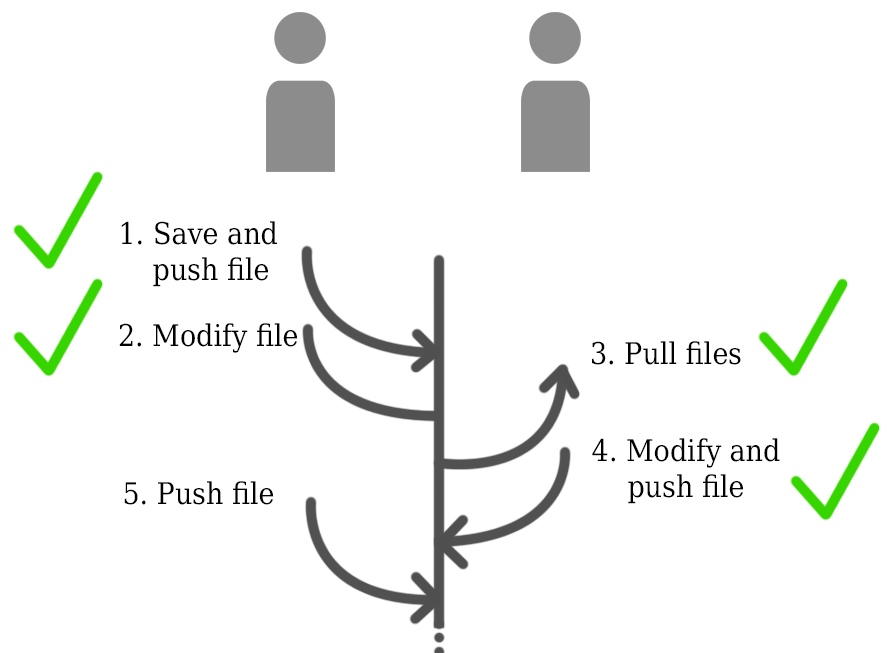
\includegraphics[width=0.9\textwidth]{VCS4}
	\end{figure}
	
}

\frame{ 
	\frametitle{Why do you want to use it?}
	
	\begin{figure}[hbtp]
		\centering
		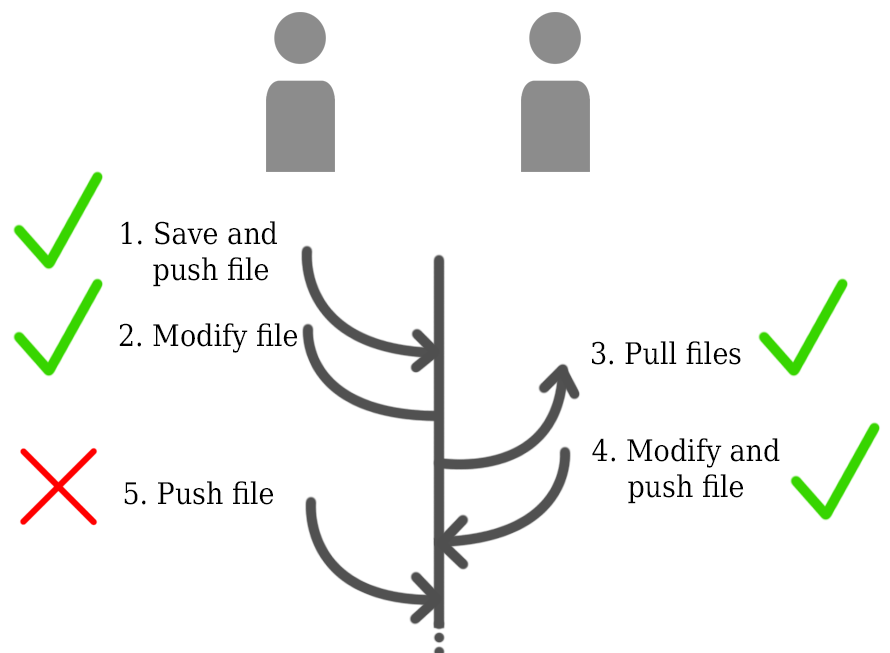
\includegraphics[width=0.9\textwidth]{VCS5}
	\end{figure}
	
}


\subsection{Merge}
\frame{ 
	\frametitle{Merge}
When conflicts occur they must be solved one way or another.
The most common way is to merge files.
\\
This is taking what was in the original file, the modified, compare them and bring the correct output.
	\begin{figure}[hbtp]
	\centering
	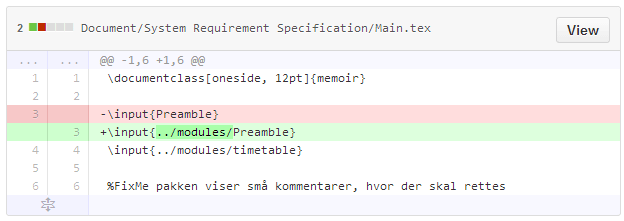
\includegraphics[width=0.95\textwidth]{Merge}
	\end{figure}
}


\section{How to get started}

\frame{
	\frametitle{How to get started}	
	
To get setup and running we will need the following:

\begin{itemize}
	\item Create a GitHub account.
	\item Download and install SmartGit.
	\item Setup SmartGit with GitHub.
	\item Create a small collaborate example.
\end{itemize}
}

\subsection{Create a GitHub account}
\frame{
\frametitle{Create a GitHub account}	

\begin{itemize}
	\item Go to \url{github.com}
	
	\item Create a user.
	\item[] Remember -- this name will be visible.
	
	\item Select a free plan. 
	
\end{itemize}
	
}

\subsection{Download and install SmartGit}

\frame{
\frametitle{Download and install SmartGit}

\begin{itemize}
	\item Download SmartGit from \url{http://www.syntevo.com/smartgit/download}
	\item Install SmartGit with the standard settings.
\end{itemize}	
}

\subsection{Setup SmartGit with GitHub.}

\frame{
	\frametitle{Setup SmartGit with GitHub.}
	
	\begin{itemize}
		\item Open the program.
		\item Select "Non-commercial use only".
		\item[] Confirm this.
		\item Select the second option for SSH with Git.
		\begin{itemize}
			\item Enter your GitHub account name.
			\item Click the "Generate API Token" key.
			\item Feel free whether to use a master password or not.
			\item[] It's security and will promt you after each reboot.
		\end{itemize}
		\item Finish the setup.

	\end{itemize}	
}

\frame{
	\frametitle{Setup SmartGit with GitHub.}
	
	\begin{itemize}
		\item Close the pop up menu.
		\item Select from the menu bar \texttt{Tools} $\rightarrow$ 
		\texttt{Open Git-Shell}.
		\item Follow the link from step 1 with the Git-shell as terminal. 
		\\
		\textbf{DO NOT DOWNLOAD THE NATIVE APP}.
	\end{itemize}
	\url{https://help.github.com/articles/generating-ssh-keys}
		
}

\section{Setup a Repository (single project)}
\frame{
	\frametitle{Setup a Repository (single project)}
	
	\begin{itemize}
		\item Go to \url{github.com} and login.
		\item Select \texttt{+New Repository}
	\end{itemize}		
	
	\begin{figure}[hbtp]
		\centering
		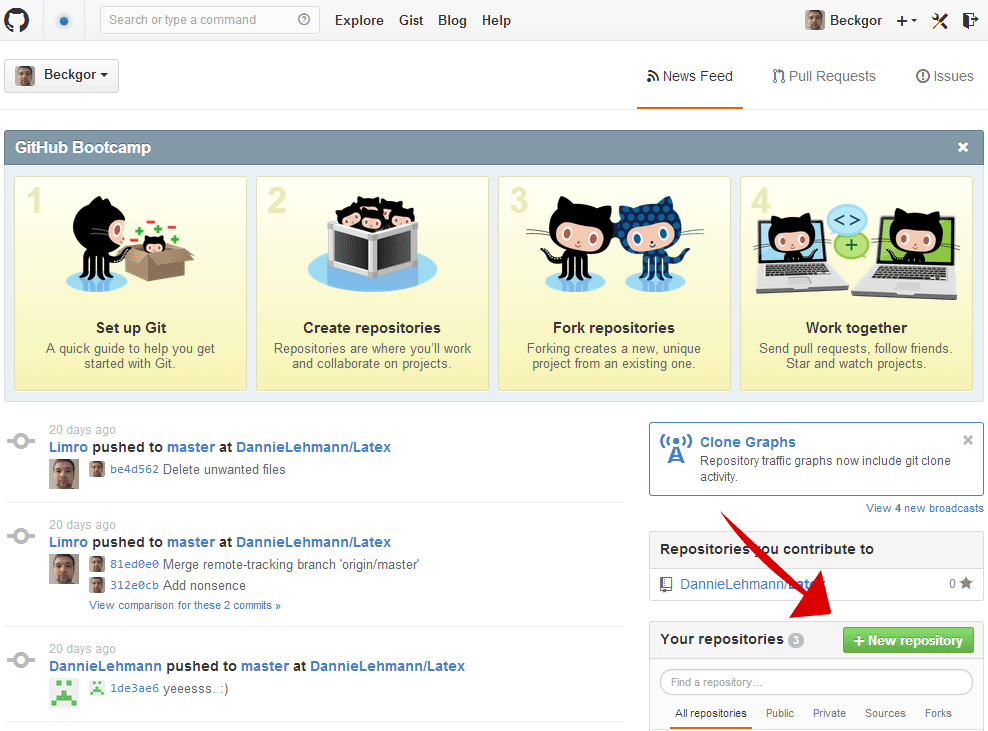
\includegraphics[width=0.95\textwidth]{Repo1}
	\end{figure}
}
		
		
\frame{
	\frametitle{Setup a Repository (single project)}
	
	\begin{itemize}
		\item Create a name for the repository.
		\item (Optional) Add a .gitignore (more of this later).
	\end{itemize}		
	
	\begin{figure}[hbtp]
		\centering
		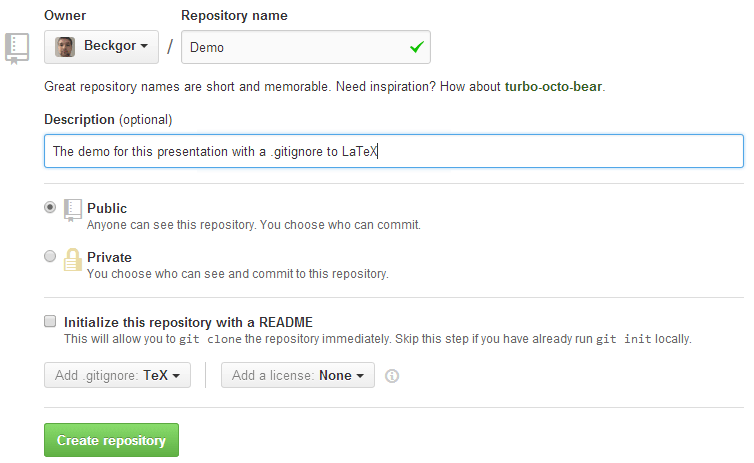
\includegraphics[width=0.95\textwidth]{Repo2}
	\end{figure}
}

\frame{
	\frametitle{Setup a Repository (single project)}
	
	There you go -- no so hard.		
	
	\begin{figure}[hbtp]
		\centering
		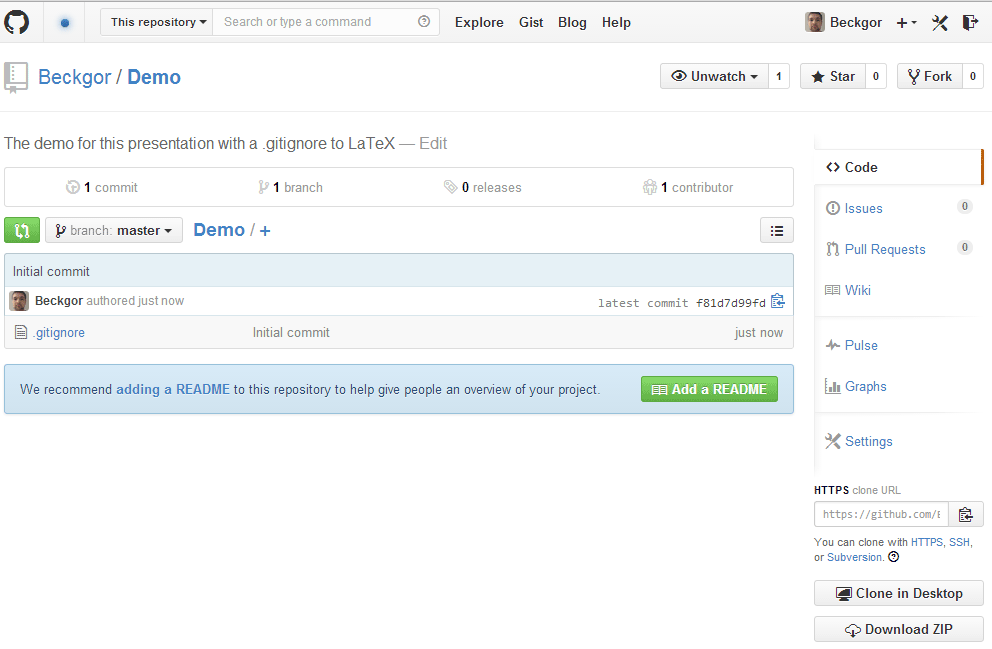
\includegraphics[width=0.95\textwidth]{Repo3}
	\end{figure}
}


\section{Add collaborators (single project)}
\frame{
	\frametitle{Add collaborators (single project)}
	
	\begin{itemize}
		\item Hit \texttt{Settings} in the right pane.
		\item Select \texttt{+New Repository}
		\item Select \texttt{Collaborators}
		\item Enter a username
	\end{itemize}		
	
	\begin{figure}[hbtp]
		\centering
		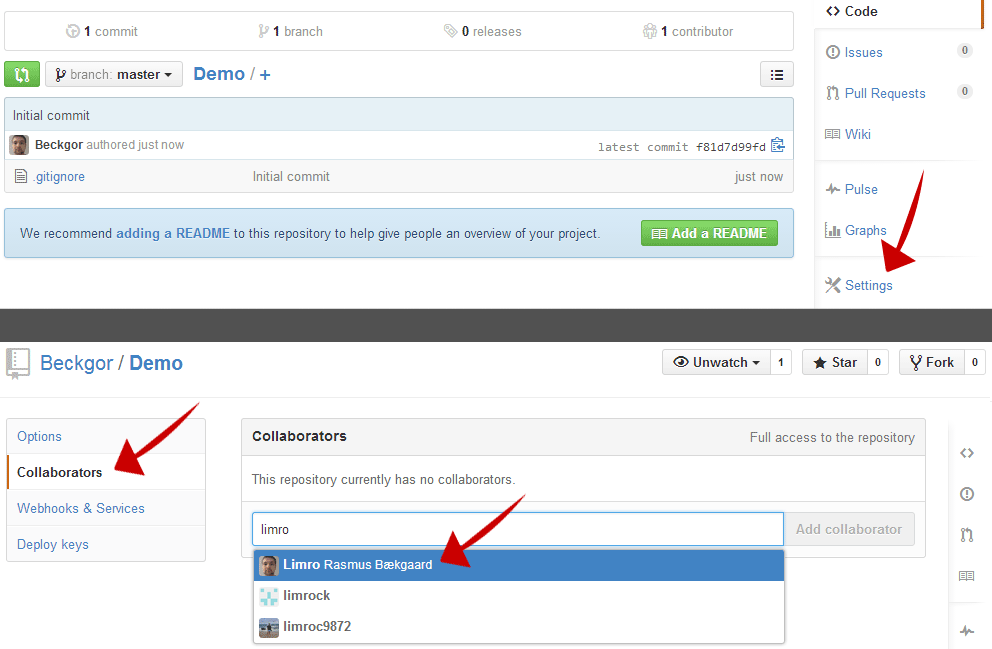
\includegraphics[width=0.85\textwidth]{Add1}
	\end{figure}
}

\section{Setup a Repository (multiple projects)}
\frame{
	\frametitle{Setup a Repository (multiple projects)}
	
	\begin{itemize}
		\item You want this if you know who you work with over multiple 
		projects / assignments and need multiple repositories.
		\item Go to the front page, click your user name and select 
		\texttt{Create organization}.
	\end{itemize}		
	
	\begin{figure}[hbtp]
		\centering
		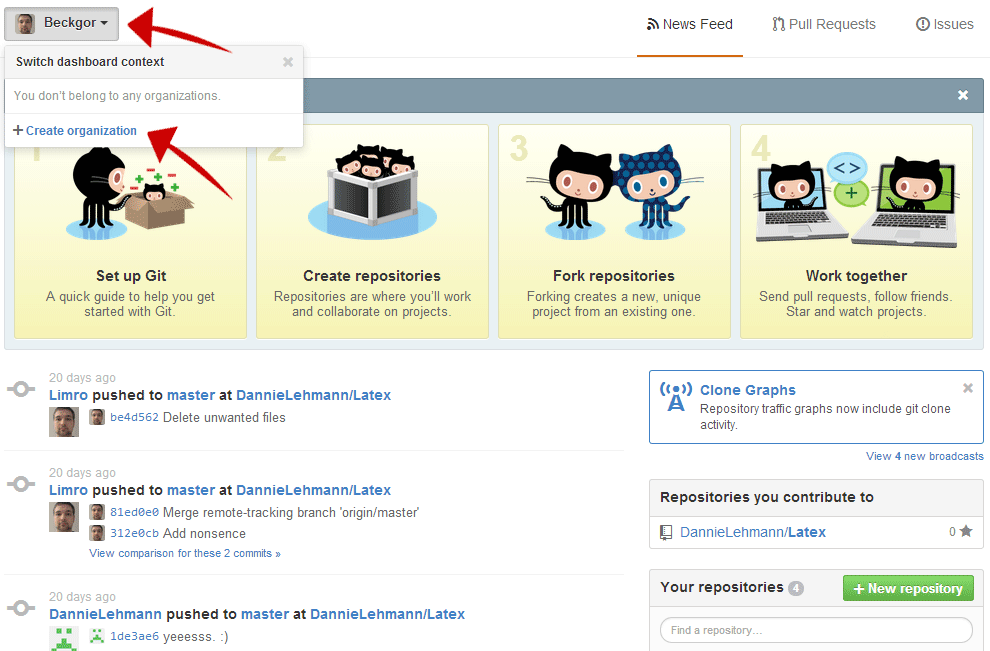
\includegraphics[width=0.95\textwidth]{Org1}
	\end{figure}
}

\frame{
	\frametitle{Setup a Repository (multiple projects)}
	
	\begin{itemize}
		\item Select a name and give your mail-address.
	\end{itemize}		
	
	\begin{figure}[hbtp]
		\centering
		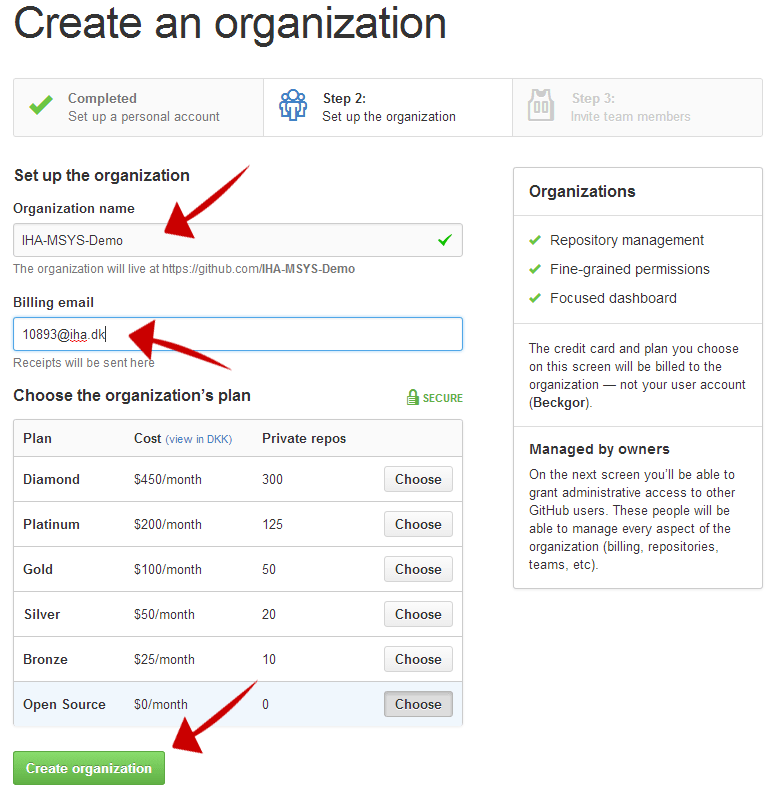
\includegraphics[width=0.65\textwidth]{Org2}
	\end{figure}
}

\frame{
	\frametitle{Setup a Repository (multiple projects)}
	
	\begin{itemize}
		\item Invite members (can be done later as well).
	\end{itemize}		
	
	\begin{figure}[hbtp]
		\centering
		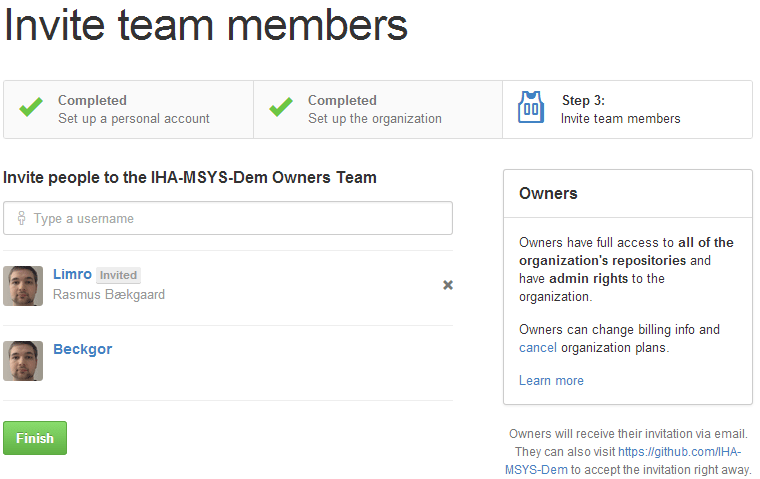
\includegraphics[width=0.95\textwidth]{Org3}
	\end{figure}
}

\subsection{Invite members to organization}
\frame{
	\frametitle{Setup a Repository (multiple projects)}
	
	\begin{itemize}
		\item Go to the front page.
		\item Select your organization.
		\item Hit \texttt{View <name>}.
	\end{itemize}		
	
	\begin{figure}[hbtp]
		\centering
		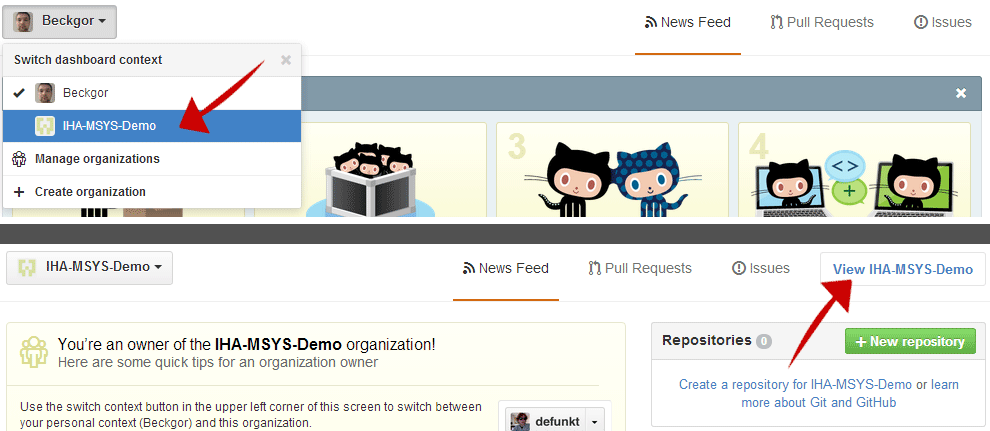
\includegraphics[width=0.95\textwidth]{Org4}
	\end{figure}
}

\frame{
	\frametitle{Setup a Repository (multiple projects)}
	
	\begin{itemize}
		\item Go to the front page.
		\item Select your organization.
		\item Hit \texttt{View <name>}.
	\end{itemize}		
	
	\begin{figure}[hbtp]
		\centering
		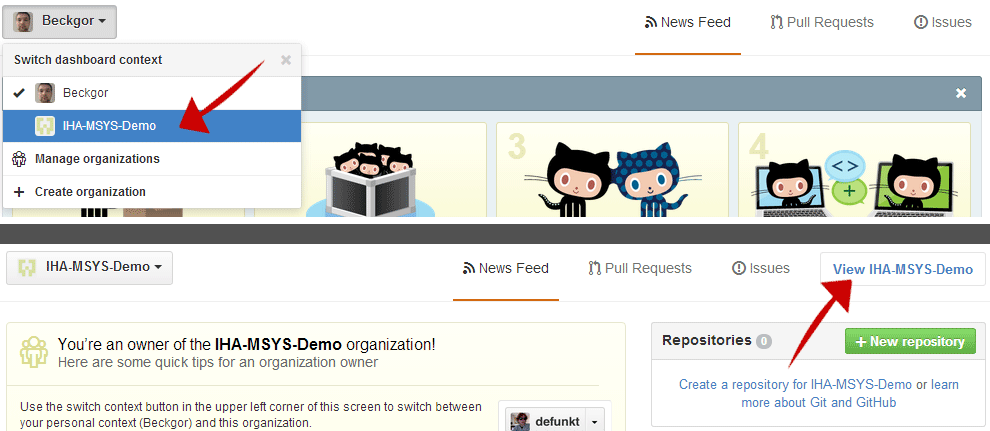
\includegraphics[width=0.95\textwidth]{Org4}
	\end{figure}
}




%\section{Live demo}
%\frame{
%\frametitle{Live demo}
%
%Time for showing how this work.
%We will go through the following:
%
%\begin{itemize}
%	\item Create a repository (project).
%	\item Add collaborators to the repository.
%	\item Add files to the repository, modify and push them (upload).
%	\item Create a merge conflict and solve it properly.
%	\item Create a list of files to ignore.
%\end{itemize}
%}



\end{document}

